\chapter{Performance Simulation Environment}
\label{chapter:performance-simulation-environment}

This chapter describes a more detailed view of modeling and simulation framework, Performance Simulation Environment (PSE), and its usage for performance analysis of a packet processing system. We begin with an overview of PSE concepts and tools, and continue by describing the three components of a PSE model. After that, we go through the simulation and monitoring of PSE applications.

\section{Toolset Overview}
\label{sec:toolset-overview}

PSE is a toolset and simulation environment for dynamic performance analysis of, initially designed but not limited to, parallel computing systems. The tools consist of graphical model editors, compiler tools, and discrete event simulator runtime. Figure~\ref{fig:pse-toolset} depicts the organization of the PSE tools.

\begin{figure}[]
  \begin{center}
    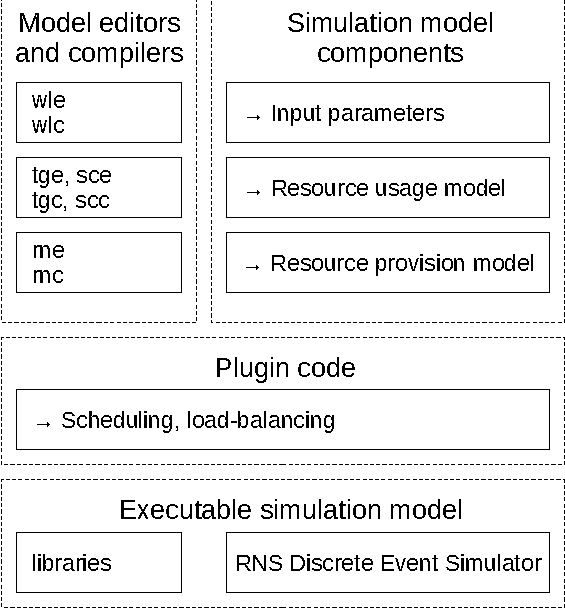
\includegraphics[width=0.5\textwidth]{images/pse-toolset-overview.pdf}
    \caption{PSE toolset includes the model editors, compiler tools and the simulator runtime libraries.}
    \label{fig:pse-toolset}
  \end{center}
\end{figure}

The graphical model editors -- workload editor, wle; task graph editor, tge; sequence chart editor, sce; and resource network editor, rne -- are used to build and edit the PSE model representation of a system. Each model editor has a corresponding compiler (wlc, tgc, scc, and rnc, respectively), which is used to compile the textual model representations into C-code. % Plugin code can be used to determine custom scheduling and load-balancing algorithms.

Figure~\ref{fig:pse-compile-workflow} presents the workflow from the modeling into an executable simulation model. First, the graphical editors are used to describe the model components. These components are then compiled into C-code using PSE compilers. Finally, the compiled C-files and the built-in simulator runtime libraries are compiled into an executable simulator program, using generic C compiler such as GCC~\cite{stallman:2009:gcc}. The resulting program can be run on top of Linux operating system on commodity hardware.

\begin{figure}[]
  \begin{center}
    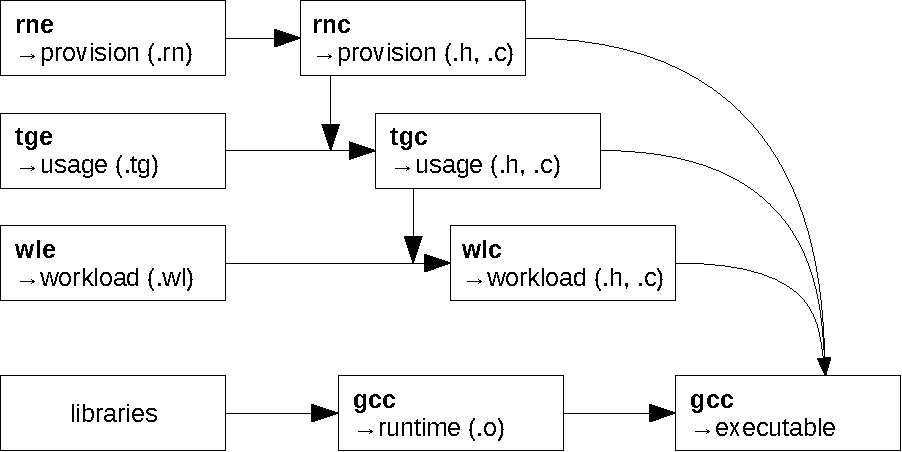
\includegraphics[width=0.75\textwidth]{images/pse-compile-workflow.pdf}
    \caption{PSE compilation workflow.}
    \label{fig:pse-compile-workflow}
  \end{center}
\end{figure}

\section{PSE Model}
PSE models the system under study as a resource network. The complete model consists of three main components: resource provision model, resource usage model and workload model. Each of the components is presented as directed graphs, where the nodes represent model entities and the arcs represent the possible flow directions of the tasks.

The resource provision model represents the available system resources, for example computer hardware. The graph nodes represent resource entities, and arcs represent the possible usage order of the resources. The resources are consumed by the tasks, generated by the workload model and guided by the resource usage model.

Figure~\ref{fig:resource-provision-model} presents an example of a resource provision model. The model is from PSE's example experiment~\cite{Hanhirova:2014:PSE} setup, where vehicles communicate with a cloud datacenter through LTE base stations and core network. There are six resource nodes, representing the vehicle CPU and LTE resources, the LTE basestation's evolved node B~\cite{Sesia:2009:LTE} (eNb) CPU and communication resources, and the core network and server resources.

\begin{figure}[]
  \begin{center}
    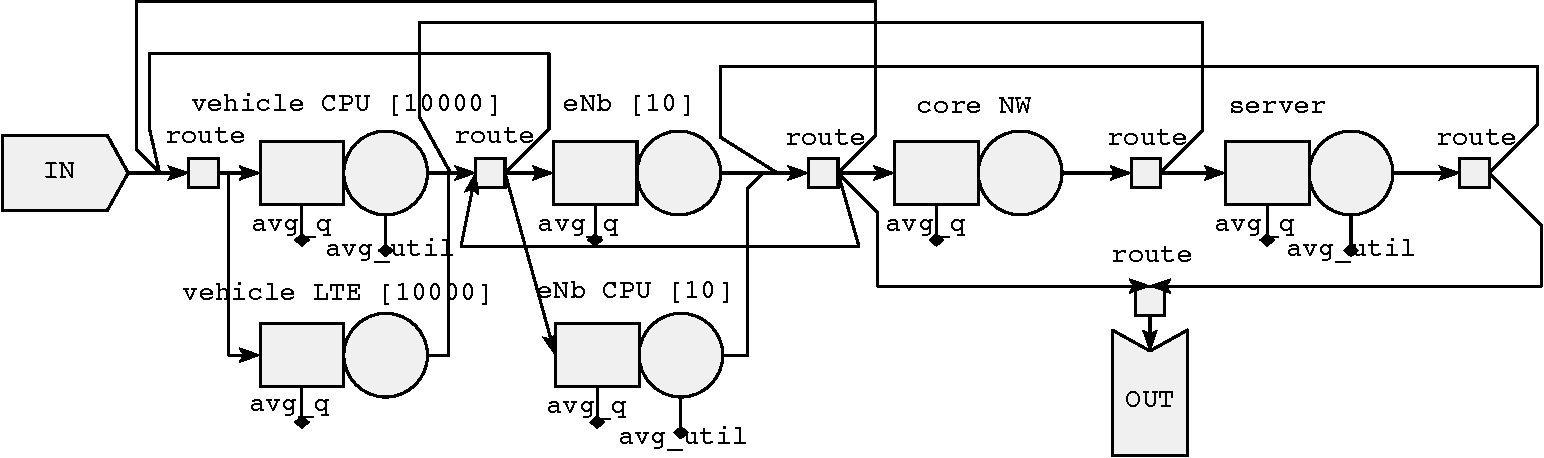
\includegraphics[width=\textwidth]{images/pse-models/pse-rn-example.pdf}
    \caption{An example of resource provision model from a vehicle communication experiment. The model contains six active resource nodes presenting the resources needed for the communication between the vehicles and the cloud datacenter. The probes are used to gather data from the simulation. Figure from~\cite{Hanhirova:2014:PSE}}
    \label{fig:resource-provision-model}
  \end{center}
\end{figure}

A resource can be either active or passive. Active resources provide service and introduce service delay to the tasks using them. An example of active resource could be a processor core, which can serve certain amount of processing cycles per unit time. Passive resources do not induce direct delay to the jobs, but their possession is required to access certain other resources. Memory partitions could be an example of passive resource. The example in the Figure~\ref{fig:resource-provision-model} contains only active resources.

The resource usage models can be presented as message sequence charts or tasks graphs. We omit the discussion of the sequence chart in this thesis. Task graph is a presentation of the resource usage of the tasks arriving to the system. The nodes in the task graph can be divided into three categories: execution nodes describe the resource usage events and activities, branching nodes conditionally guide the tasks through the graph, and fork/join nodes present task subdivision. The arcs present the flow of control in the system.

Figure~\ref{fig:resource-usage-model} presents the resource usage model of the vehicle example presented above. The rectangle nodes consume the resources from the resource provision model presented in the Figure~\ref{fig:resource-provision-model}. The branching nodes are presented as the parallelograms. Note that only one of the paths are take after each of the parallelogram.

\begin{figure}[]
  \begin{center}
    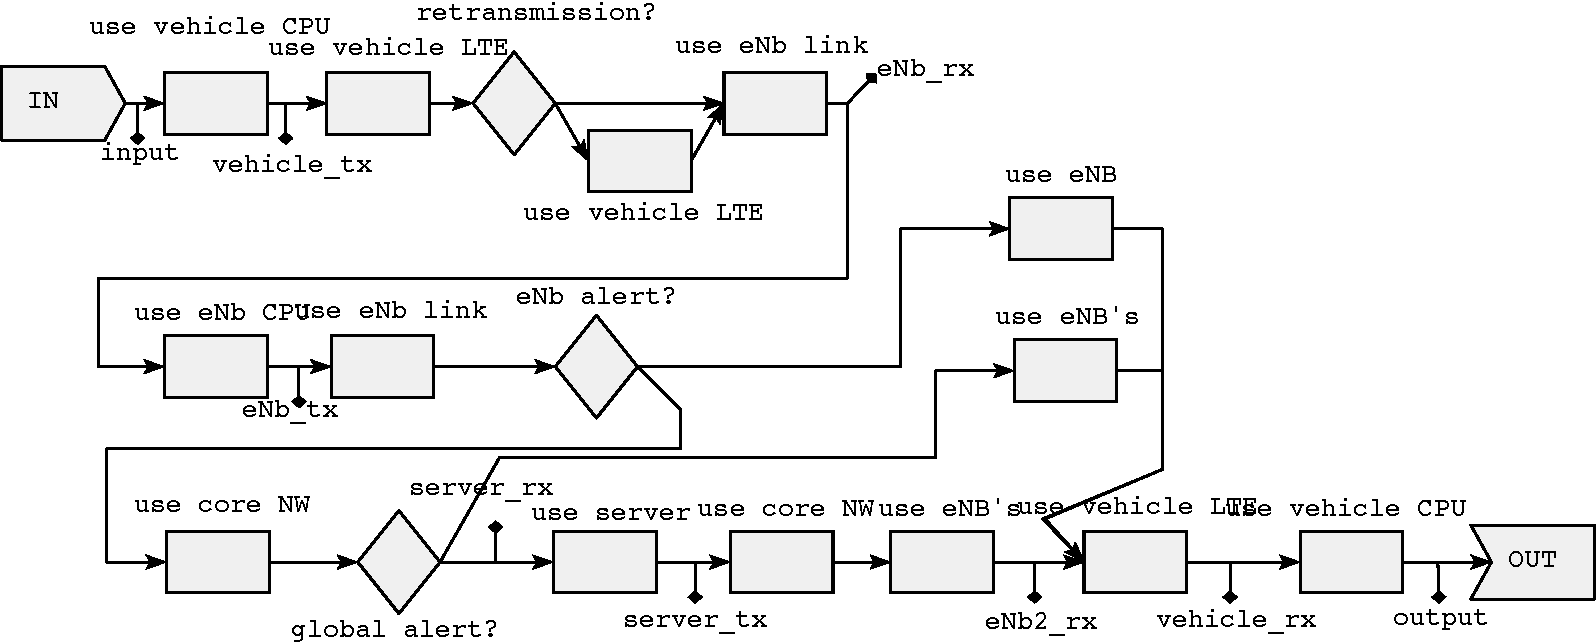
\includegraphics[width=\textwidth]{images/pse-models/pse-tg-example.pdf}
    \caption{An example of resource usage model from a vehicle communication experiment. The rectangles present resource usage nodes. Figure from~\cite{Hanhirova:2014:PSE}}
    \label{fig:resource-usage-model}
  \end{center}
\end{figure}

The workload model generates tasks, which traverse through the system according to the rules defined in the resource usage model, consuming the resources defined in the resource provision model. The nodes in the workload graph describe the task generating processes, and the arcs define the relationships between them. The graph representing the workload model must be acyclic.

The event spawn rate can be constant or random (specified for example with probability distribution). When an event is spawned, it progresses through the resource provision model triggering the resource usages, thus getting delayed.

\begin{figure}[]
  \begin{center}
    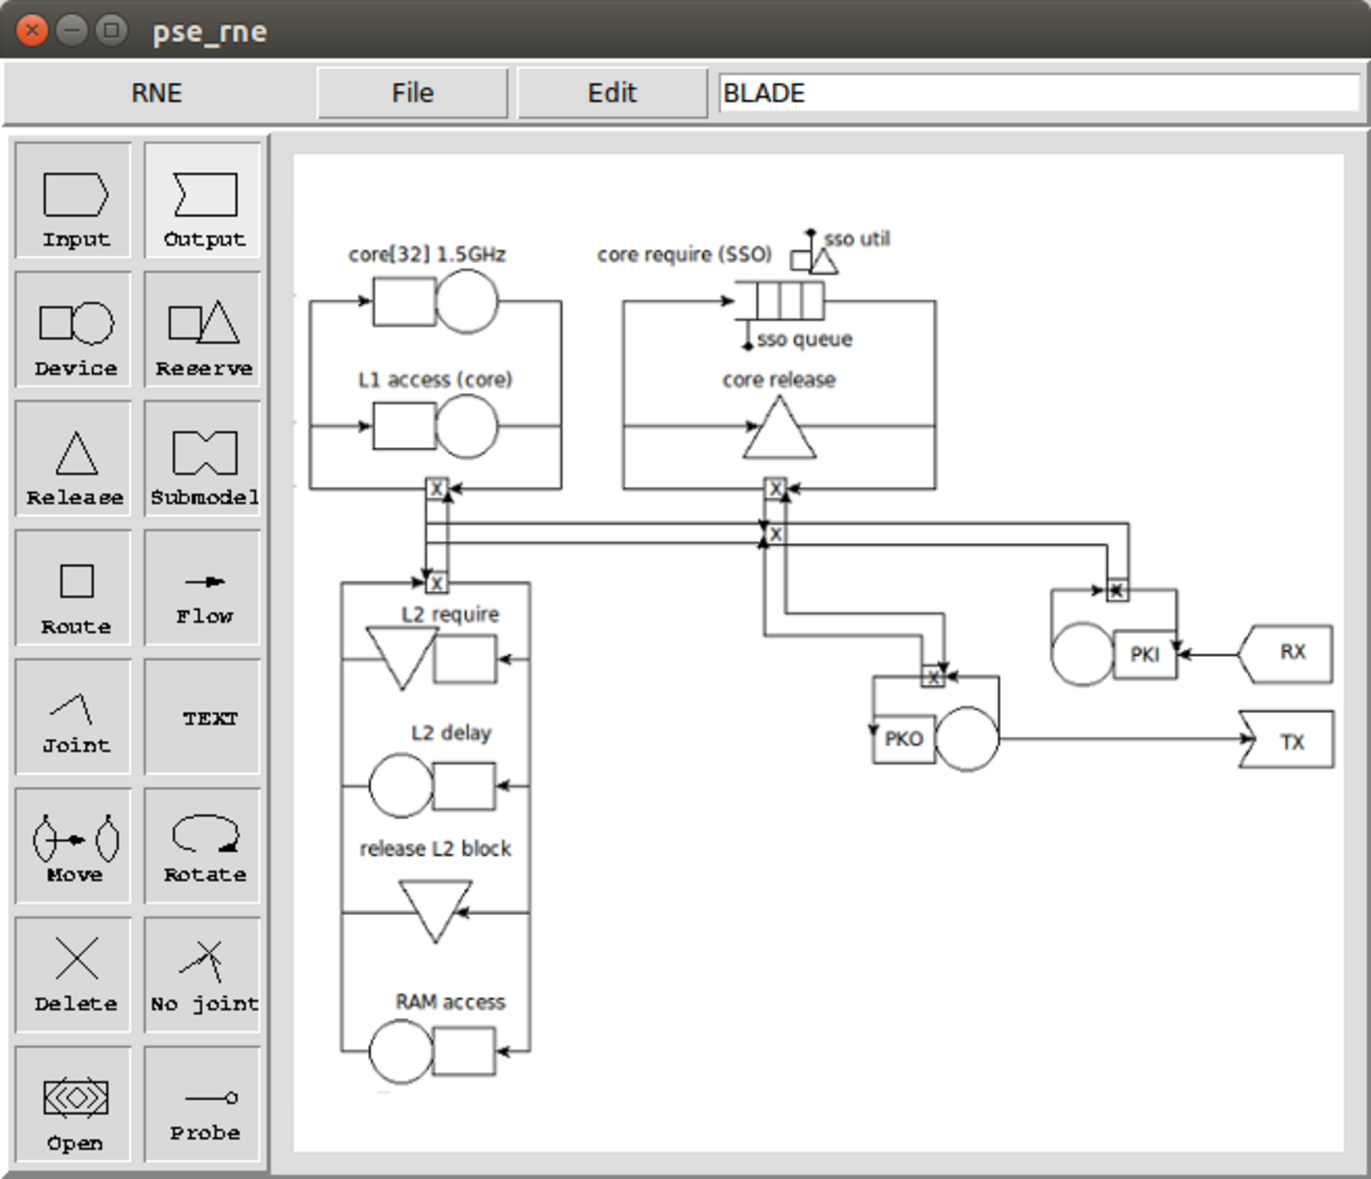
\includegraphics[width=0.6\textwidth]{images/rne-example.pdf}
    \caption{The graphical user interface of the resource network editor. The actual resource network model is presented in the middle, and the toolbar on the left.}
    \label{fig:rne-example}
  \end{center}
\end{figure}

\section{Monitoring}

PSE has flexible, built-in, monitoring support, which offers both trace-based and on-the-fly monitoring. The monitoring is controlled by attaching probes to the nodes and vertices of the simulation model nodes. It can be done on all the three model levels and practically every simulation system state change can be captured. There are essentially two different types of probes in PSE: the trace probes for trace-based measurements, and the metric probes for on-the-fly measurements.

In the resource provision model, the probes can be attached to two different parts of the resource, to measure either the resource utilization, or its queue size. The trace probes capture every change in the resource utilization or queue size, whereas the metric trace produce aggregate only the descriptive statistics. The descriptive statistics currently include mean, standard deviation, minimum, maximum, sum, and total number of tasks that passed through.

In the resource usage model, the probes can be attached to the model edges, producing a time stamped trace whenever a task travels the edge. The timing can be either absolute time with respect to the global system time, or relative to the process start time. The metric probes can be used to capture the average times of all tasks relative to the start of the process. Probes in the workload model are used to control the grouping of the resource usage and resource provision probes.

The probe output is written in a text file defined in the probe node attributes. The trace probes write the output in Comma-Separated Values~\cite{Shafranovic:2005:CSV} format, and the metrics traces write a standard descriptive statistics output. Using the trace based probing can substantially slow down the simulation, as the output files easily grow very large, slowing down the writes. Thus, whenever the complete trace log is not needed, it is recommended to use the metric based probing. Figure~\ref{fig:full-model} in Section~\ref{sec:hardware-model} presents examples of probes attached to core-, memory- and scheduler units in the hardware model as well as the in- and out- probes in the software model.

\section{Resource Network Simulator}
\label{sec:resource-network-simulator}

Performance Simulation Environment provides a discrete event simulator engine, named resource network simulator (RNS). The final simulator program is created by compiling the RNS runtime libraries together with the generated simulation model code. The simulator engine manages the simulation execution, i.e. tracks the global simulation time, schedules tasks and manages the system monitoring.

The simulator inputs are generated by the workload model, which spawns a new system thread for each generated input. The input can be either a control input or an actual workload task. The former of these are used for the simulation control, for example changing or resetting the simulation time or monitoring metrics. The latter are the actual task entities presented in Section~\ref{sec:hardware-model}.

\subsection{Simulator Engine}
\label{sec:simulator-engine}

\begin{figure}[]
  \begin{center}
    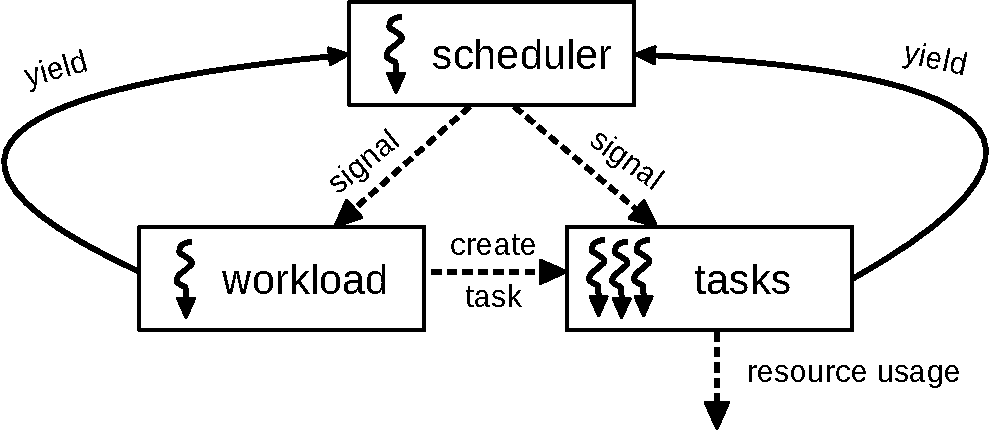
\includegraphics[width=0.5\textwidth]{images/rns-threads.pdf}
    \caption{The thread cycle of performance simulation environment's resource network simulator engine.}
    \label{fig:rns-threads}
  \end{center}
\end{figure}

Figure~\ref{fig:rns-threads} represents the model of execution in the RNS engine. The RNS scheduler, running in an infinite loop in its own thread, signals the workload threads or the task threads, based on the trigger time. RNS advances in the event-advance manner, meaning that the thread with the smallest trigger time, based on the scheduler's internal bookkeeping, gets always executed first.

The workload threads spawn new tasks to the actual task-pool, according to the code generated from the workload model. The execution of the task-pool threads advance the actual simulator, consuming the resources based on the values defined in the resource usage model. The actual code that is consumed by the threads is generated by compiling the application models with references to the workload model, hardware models and the runtime libraries. Each time a thread's task encounters an event that is dependent on the other thread's execution, it yields the execution back to the scheduler thread, which then signals the thread, again, with the smallest trigger time.

%%% Local Variables:
%%% mode: latex
%%% TeX-master: "thesis-hartikainen"
%%% End:
